\documentclass[tikz,border=6pt]{standalone}
% Shared visual language for the original benchmark atlas.
\usepackage[T1]{fontenc}
\usepackage{lmodern}
\usepackage{amsmath,amssymb}
\usetikzlibrary{arrows.meta,calc,positioning,shapes.geometric,patterns,decorations.pathmorphing,backgrounds,fit}
\definecolor{ink}{HTML}{173948}
\definecolor{flow}{HTML}{167D9A}
\definecolor{control}{HTML}{A65217}
\definecolor{measure}{HTML}{70518A}
\definecolor{pale}{HTML}{EAF2F5}
\definecolor{muted}{HTML}{526571}
\definecolor{utility}{HTML}{2E8665}
\tikzset{
  every node/.style={font=\sffamily\small,text=ink},
  equipment/.style={draw=ink,line width=1pt,fill=pale,rounded corners=2pt},
  process/.style={draw=flow,line width=1.2pt,-{Latex[length=2.5mm]}},
  signal/.style={draw=control,line width=.8pt,dashed,-{Latex[length=2mm]}},
  util/.style={draw=utility,line width=1pt,-{Latex[length=2.2mm]}},
  dimension/.style={draw=muted,line width=.6pt,{Latex[length=1.7mm]}-{Latex[length=1.7mm]}},
  labelbox/.style={fill=white,inner sep=2pt,font=\sffamily\footnotesize,align=center},
  annotation/.style={font=\sffamily\footnotesize,text=muted,align=left},
  panel/.style={draw=ink!20,fill=ink!2,rounded corners=3pt,inner sep=6pt},
  instrument/.style={circle,draw=measure,fill=white,line width=.8pt,minimum size=8mm,inner sep=1pt,font=\sffamily\scriptsize,align=center},
  port/.style={circle,fill=flow,inner sep=1.6pt},
  box/.style={equipment,minimum width=3cm,minimum height=1cm,align=center},
}
\newcommand{\atlasheader}[3]{%
  \node[anchor=north west,font=\sffamily\bfseries\LARGE] at (0,0) {#1};%
  \node[anchor=north west,font=\sffamily\small,text=muted] at (0,-.75) {Paper section #2: \textit{#3}};%
  \draw[ink!25,line width=.7pt] (0,-1.25)--(26,-1.25);%
}
\newcommand{\atlasfooter}[1]{%
  \draw[ink!25,line width=.5pt] (0,-15.8)--(26,-15.8);%
  \node[anchor=north west,annotation,text width=25.8cm] at (0,-16) {#1\\Original explanatory drawing. Source: Kroll \& Schulte (2014), DOI: 10.1016/j.asoc.2014.08.034. Model variants are identified in the accompanying case sheet.};%
}

\begin{document}
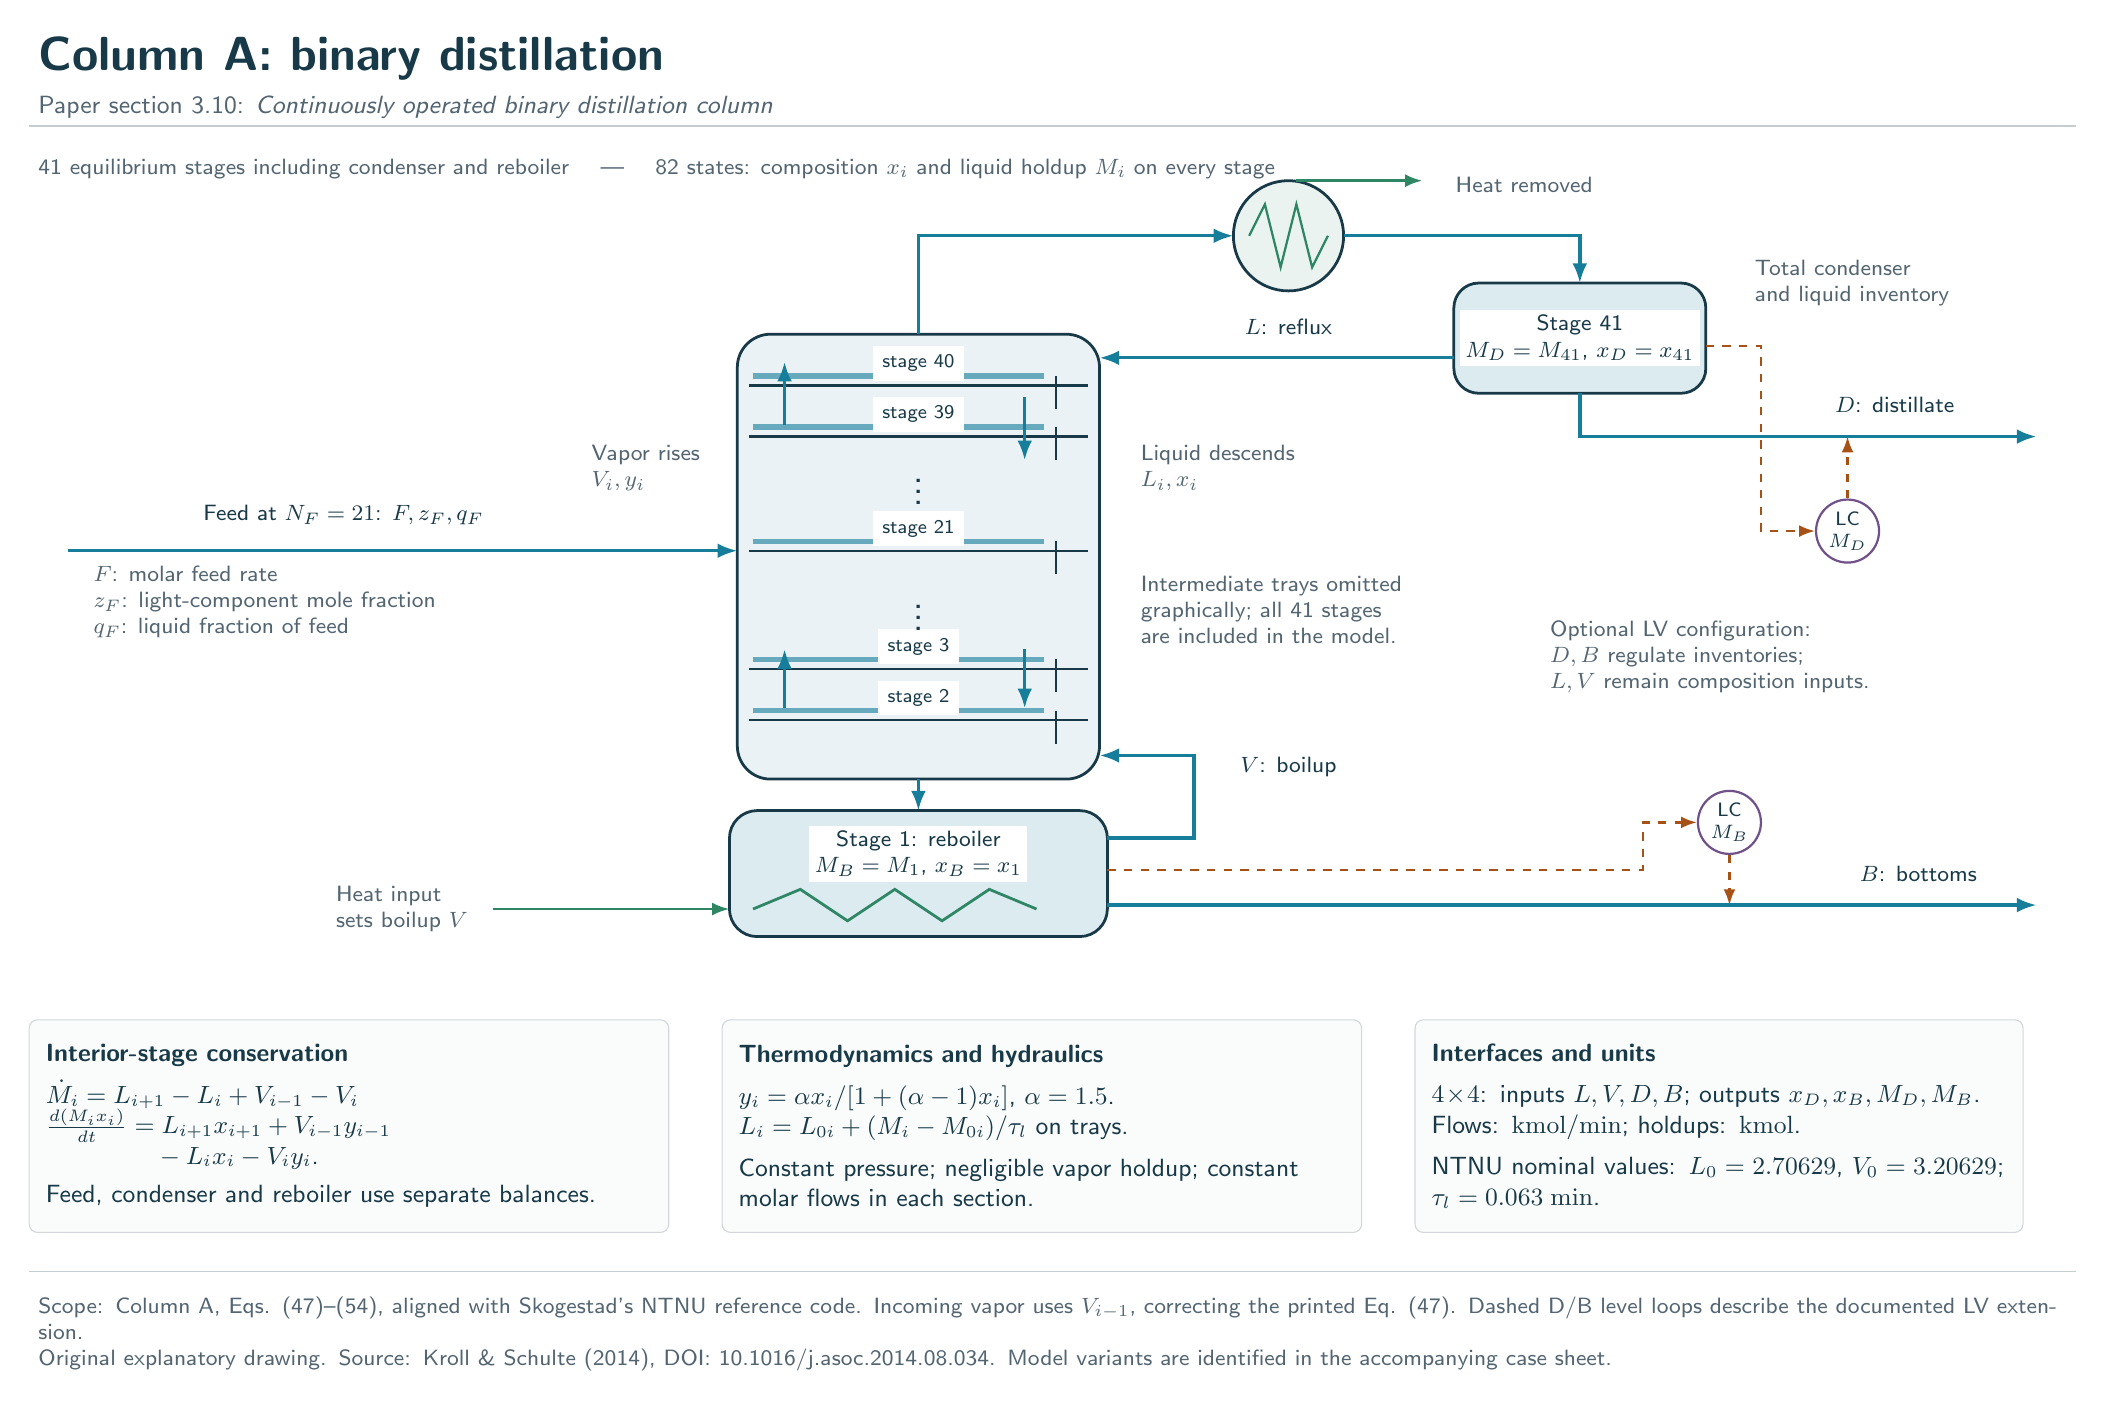
\begin{tikzpicture}[x=1cm,y=1cm]
\atlasheader{Column A: binary distillation}{3.10}{Continuously operated binary distillation column}
\node[annotation,anchor=west] at (0,-1.8) {41 equilibrium stages including condenser and reboiler \quad | \quad 82 states: composition $x_i$ and liquid holdup $M_i$ on every stage};
% Main shell: interior trays are selected to keep the diagram readable.
\draw[equipment,rounded corners=12pt] (9,-3.9) rectangle (13.6,-9.55);
\foreach \yy/\num in {-4.55/40,-5.2/39,-6.65/21,-8.15/3,-8.8/2} {
  \draw[ink,line width=.8pt] (9.15,\yy)--(13.45,\yy);
  \draw[flow!65,line width=2pt] (9.2,{\yy+.12})--(12.9,{\yy+.12});
  \draw[ink,line width=.6pt] (13.05,{\yy+.12})--(13.05,{\yy-.3});
  \node[font=\sffamily\scriptsize,fill=white] at (11.3,{\yy+.28}) {stage \num};
}
\node[font=\sffamily\Large] at (11.3,-5.8) {$\vdots$};
\node[font=\sffamily\Large] at (11.3,-7.4) {$\vdots$};
\draw[process] (9.6,-5.05)--(9.6,-4.25);
\draw[process] (9.6,-8.65)--(9.6,-7.9);
\draw[process] (12.65,-4.7)--(12.65,-5.5);
\draw[process] (12.65,-7.9)--(12.65,-8.65);
\node[annotation,anchor=east] at (8.65,-5.6) {Vapor rises\\$V_i,y_i$};
\node[annotation,anchor=west] at (14,-5.6) {Liquid descends\\$L_i,x_i$};
\node[annotation,anchor=west] at (14,-7.4) {Intermediate trays omitted\\graphically; all 41 stages\\are included in the model.};
% Feed at stage 21: composition and liquid fraction are disturbances.
\draw[process] (.5,-6.65)--(9,-6.65);
\node[labelbox] at (4,-6.2) {Feed at $N_F=21$: $F,z_F,q_F$};
\node[annotation,anchor=west] at (.7,-7.3) {$F$: molar feed rate\\$z_F$: light-component mole fraction\\$q_F$: liquid fraction of feed};
% Total condenser and accumulator are one modeled stage 41.
\draw[process] (11.3,-3.9)--(11.3,-2.65)--(15.3,-2.65);
\draw[equipment,fill=utility!10] (16,-2.65) circle[radius=.7];
\draw[utility,line width=.8pt] (15.5,-2.65)--(15.7,-2.25)--(15.9,-3.05)--(16.1,-2.25)--(16.3,-3.05)--(16.5,-2.65);
\draw[util] (16.1,-1.95)--(17.7,-1.95);
\node[annotation,anchor=west] at (18,-2) {Heat removed};
\draw[process] (16.7,-2.65)--(19.7,-2.65)--(19.7,-3.25);
\draw[equipment,fill=flow!15,rounded corners=9pt] (18.1,-3.25) rectangle (21.3,-4.65);
\draw[flow] (18.2,-3.85)--(21.2,-3.85);
\node[labelbox,align=center] at (19.7,-3.95) {Stage 41\\$M_D=M_{41}$, $x_D=x_{41}$};
\node[annotation,anchor=west] at (21.8,-3.25) {Total condenser\\and liquid inventory};
\draw[process] (19.7,-4.65)--(19.7,-5.2)--(25.5,-5.2);
\node[labelbox] at (23.7,-4.8) {$D$: distillate};
\draw[process] (18.1,-4.2)--(14.4,-4.2)--(13.6,-4.2);
\node[labelbox] at (16,-3.8) {$L$: reflux};
% Bottom stage is a reboiler, with liquid product and upward boilup.
\draw[process] (11.3,-9.55)--(11.3,-9.95);
\draw[equipment,fill=flow!15,rounded corners=10pt] (8.9,-9.95) rectangle (13.7,-11.55);
\node[labelbox,align=center] at (11.3,-10.5) {Stage 1: reboiler\\$M_B=M_1$, $x_B=x_1$};
\draw[utility,line width=1pt] (9.2,-11.2)--(9.8,-10.95)--(10.4,-11.35)--(11,-10.95)--(11.6,-11.35)--(12.2,-10.95)--(12.8,-11.2);
\draw[util] (5.9,-11.2)--(8.9,-11.2);
\node[annotation,anchor=east] at (5.7,-11.2) {Heat input\\sets boilup $V$};
\draw[process] (13.7,-10.3)--(14.8,-10.3)--(14.8,-9.25)--(13.6,-9.25);
\node[labelbox] at (16,-9.4) {$V$: boilup};
\draw[process] (13.7,-11.15)--(25.5,-11.15);
\node[labelbox] at (24,-10.75) {$B$: bottoms};
% Optional inventory controllers: D/B regulate inventories in LV structure.
\node[instrument] (lcd) at (23.1,-6.4) {LC\\$M_D$};
\draw[signal] (21.3,-4.05)--(22,-4.05)--(22,-6.4)--(lcd.west);
\draw[signal] (lcd.north)--(23.1,-5.2);
\node[instrument] (lcb) at (21.6,-10.1) {LC\\$M_B$};
\draw[signal] (13.7,-10.7)--(20.5,-10.7)--(20.5,-10.1)--(lcb.west);
\draw[signal] (lcb.south)--(21.6,-11.15);
\node[annotation,anchor=west] at (19.2,-8) {Optional LV configuration:\\$D,B$ regulate inventories;\\$L,V$ remain composition inputs.};
\node[panel,anchor=north west,text width=7.7cm,minimum height=2.7cm,align=left] at (0,-12.6) {\textbf{Interior-stage conservation}\\[4pt]
 $\dot M_i=L_{i+1}-L_i+V_{i-1}-V_i$\\
 $\frac{d(M_ix_i)}{dt}=L_{i+1}x_{i+1}+V_{i-1}y_{i-1}$\\$\hphantom{\frac{d(M_ix_i)}{dt}=} -L_ix_i-V_iy_i$.\\[3pt]
 Feed, condenser and reboiler use separate balances.};
\node[panel,anchor=north west,text width=7.7cm,minimum height=2.7cm,align=left] at (8.8,-12.6) {\textbf{Thermodynamics and hydraulics}\\[4pt]
 $y_i=\alpha x_i/[1+(\alpha-1)x_i]$, $\alpha=1.5$.\\
 $L_i=L_{0i}+(M_i-M_{0i})/\tau_l$ on trays.\\[4pt]
 Constant pressure; negligible vapor holdup; constant molar flows in each section.};
\node[panel,anchor=north west,text width=7.3cm,minimum height=2.7cm,align=left] at (17.6,-12.6) {\textbf{Interfaces and units}\\[4pt]
 $4\!\times\!4$: inputs $L,V,D,B$; outputs $x_D,x_B,M_D,M_B$.\\
 Flows: $\mathrm{kmol/min}$; holdups: $\mathrm{kmol}$.\\[4pt]
 NTNU nominal values: $L_0=2.70629$, $V_0=3.20629$; $\tau_l=0.063\;\mathrm{min}$.};
\atlasfooter{Scope: Column A, Eqs. (47)--(54), aligned with Skogestad's NTNU reference code. Incoming vapor uses $V_{i-1}$, correcting the printed Eq. (47). Dashed D/B level loops describe the documented LV extension.}
\end{tikzpicture}
\end{document}
